\section{definition14-3(intergenerator sheaf)}
\begin{definition}
\end{definition}

We define a special sheaf, called intergenerator sheaf, a intergeneram on $n$ strands inductively as follows: 
Suppose $n=1$, then

\begin{figure}[H] % Optional: [h] means here, [t] for top, [b] for bottom, [p] for page of floats
    \centering
    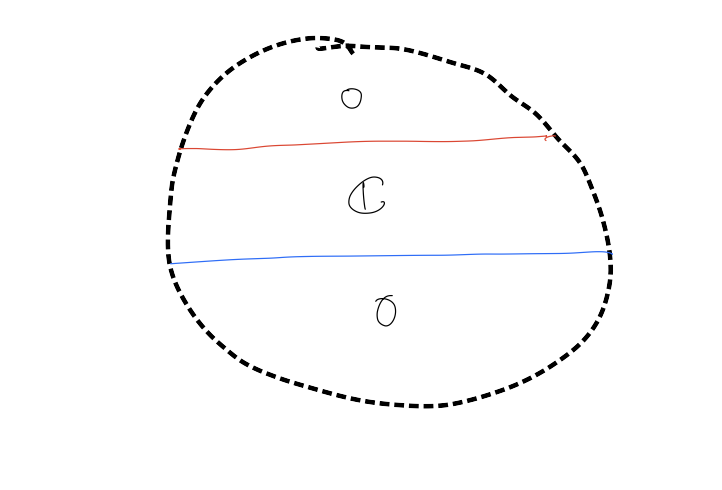
\includegraphics[width=\linewidth]{diagrams/definition14-3/1.png} % Adjust the width as needed
    \caption{Your caption here}
    \label{fig:your-label}
\end{figure}

Suppose $n>!$, then intergenerator sheaf is the unique sheaf 

\begin{figure}[H] % Optional: [h] means here, [t] for top, [b] for bottom, [p] for page of floats
    \centering
    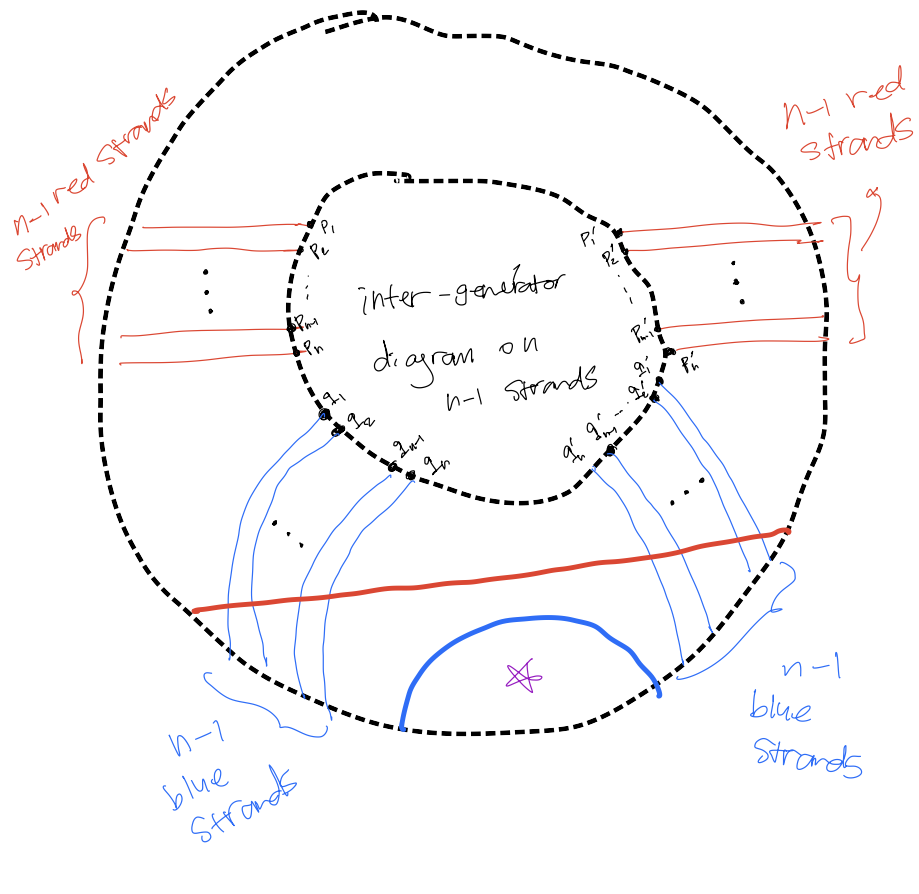
\includegraphics[width=\linewidth]{diagrams/definition14-3/2.png} % Adjust the width as needed
    \caption{Your caption here}
    \label{fig:your-label}
\end{figure}

extending the intergenerator sheaf on the intergenerator diagram on $n-1$ strands with vanishing stalk at the region containing the purple star.

(proof of well-definedness) Note that in the following diagram:

\begin{figure}[H] % Optional: [h] means here, [t] for top, [b] for bottom, [p] for page of floats
    \centering
    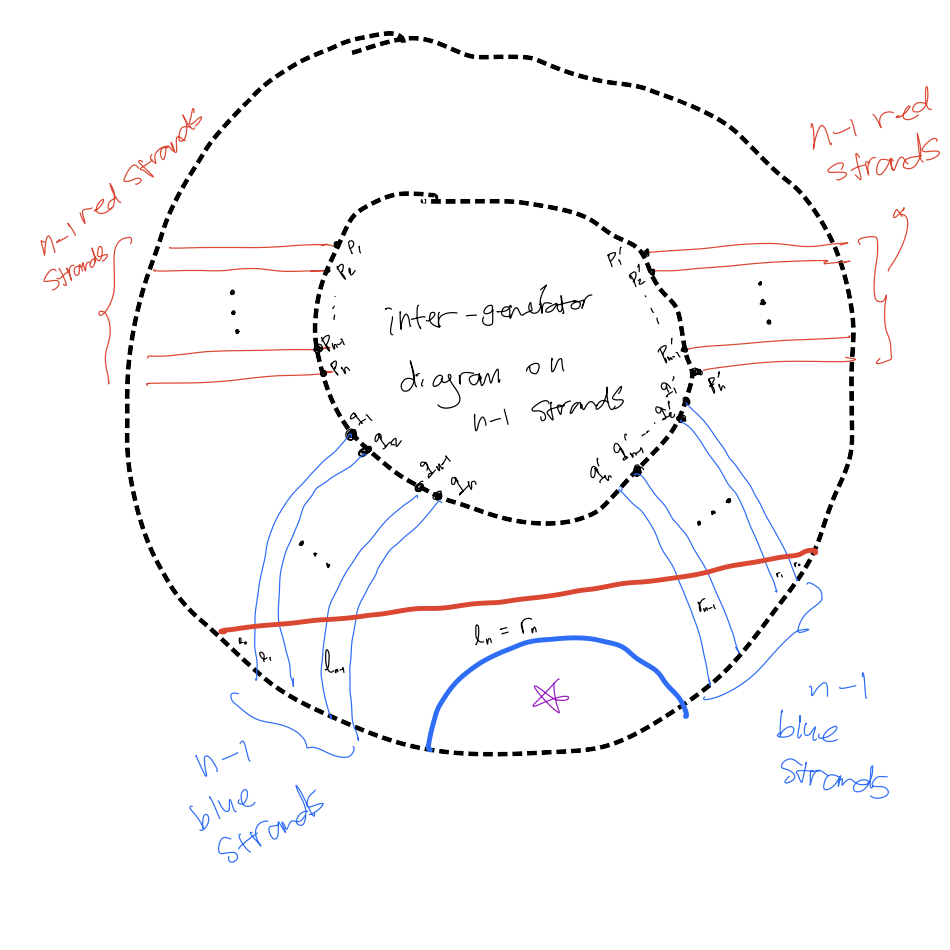
\includegraphics[width=\linewidth]{diagrams/definition14-3/3.png} % Adjust the width as needed
    \caption{Your caption here}
    \label{fig:your-label}
\end{figure}

The regions except $l_0 = r_0, l_1 - l_n, r_1 - r_n$ are connected to the regions of the intergenerator diagram on $n-1$ strands. Therefore, the stalks and the generization maps between those regions are determined. Furthermore, because the sheaf is of microlocal rank one, the stalk at $l_n = r_n$ is quasi-isomorphic to $\mathbb{C}$ and the stalk at the region bordering $l_n = r_n$ with $n^{th}$ red strand is $0$. Therefore, the stalks and generization maps between regions except $l_0 - l_{n-1}$ and $r_0 - r_{n-1}$ are determined. Now using the crossing condition to determine the stalks of $l_0 - l_{n-1}, r_0 - r_{n-1}$ by induction. Suppose the stalks and generization maps between regions except $l_0 - l_k$ and $r_0 - r_k$ are determined. Then by the crossing conditions of the crossings of the $k+1^{th}$ blue strand and the $n+1^{th}$ strand determine the stalks of $l_k$ and $r_k$ and maps into them. Therefore, the proof is complete.